\documentclass[t]{beamer}
\usepackage[utf8]{inputenc}  % to be able to type unicode text directly
%\usepackage[french]{babel}   % french typographical conventions
\usepackage{inconsolata}     % for a nicer (e.g. non-courier) tt family font
%\usepackage{amsthm,amsmath}  % fancier mathematics
\usepackage{array} % to fine-tune tabular spacing
\usepackage{bbm} % for blackboard 1

\usepackage{graphicx}        % to include images
%\usepackage{animate}         % to include animated images
\usepackage{soul}            % for colored strikethrough
%\usepackage{bbding}          % for Checkmark and XSolidBrush
\usepackage{hyperref,url}

\colorlet{darkgreen}{black!50!green}  % used for page numbers
\definecolor{term}{rgb}{.9,.9,.9}     % used for code insets

\setlength{\parindent}{0em}
\setlength{\parskip}{1em}


% coco's macros
\newcommand{\ds}{\displaystyle}
\def\R{\textbf{R}}
\def\C{\textbf{C}}
\def\K{\textbf{K}}
\def\N{\textbf{N}}
\def\F{\mathcal{F}}
\def\x{\textbf{x}}
\def\y{\mathbf{y}}
\def\u{\mathbf{u}}
\def\Z{\textbf{Z}}
\def\d{\mathrm{d}}
\DeclareMathOperator*{\argmin}{arg\,min}
\DeclareMathOperator*{\argmax}{arg\,max}
\newcommand{\reference}[1] {{\scriptsize \color{gray}  #1 }}
\newcommand{\referencep}[1] {{\tiny \color{gray}  #1 }}
\newcommand{\unit}[1] {{\tiny \color{gray}  #1 }}

% matrix groups and sets
\newcommand{\M}{\mathrm{M}}
\newcommand{\GL}{\mathrm{GL}}
\newcommand{\TS}{\mathrm{TS}}
\newcommand{\TI}{\mathrm{TI}}
\newcommand{\UU}{\mathrm{U}}
\newcommand{\OO}{\mathrm{O}}
\newcommand{\SO}{\mathrm{SO}}
\newcommand{\SU}{\mathrm{SU}}
\newcommand{\SL}{\mathrm{SL}}
\newcommand{\SSS}{\mathrm{S}}
\newcommand{\HH}{\mathrm{H}}

\newcommand{\parens}[1]{\left(#1\right)} % (x)
\newcommand{\pairing}[2]{\left\langle #1,#2\right\rangle} % <x,y>

% \abs{x}   ->    |x|
% \Abs{x}   ->   ||x||
% \ABS{x}   ->  |||x|||
\newcommand{\abs}[1]{\left|#1\right|}
\newcommand{\Abs}[1]{\left\|#1\right\|}
\newcommand{\ABS}[1]{{\left\vert\kern-0.25ex\left\vert\kern-0.25ex\left\vert #1 \right\vert\kern-0.25ex\right\vert\kern-0.25ex\right\vert}}

% disable spacing around verbatim
\usepackage{etoolbox}
\makeatletter\preto{\@verbatim}{\topsep=0pt \partopsep=0pt }\makeatother

% disable headings, set slide numbers in green
\mode<all>\setbeamertemplate{navigation symbols}{}
\defbeamertemplate*{footline}{pagecount}{\leavevmode\hfill\color{darkgreen}
   \insertframenumber{} / \inserttotalframenumber\hspace*{2ex}\vskip0pt}

%% select red color for strikethrough
\makeatletter
\newcommand\SoulColor{%
  \let\set@color\beamerorig@set@color
  \let\reset@color\beamerorig@reset@color}
\makeatother
\newcommand<>{\St}[1]{\only#2{\SoulColor\st{#1}}}
\setstcolor{red}

% make everything monospace
\renewcommand*\familydefault{\ttdefault}

\begin{document}

\begin{frame}[plain,fragile]
\LARGE
\begin{verbatim}



        ANALYSE NUMÉRIQUE 6/6

     Algèbre linéaire numérique :
         méthodes itératives



EML
30--11--2020
\end{verbatim}
\end{frame}

\begin{frame}[fragile]
PLAN\\
====

1. Aperçu des résultats principaux ({\bf 30min})

2. Travail par groupes ({\bf 90min})

3. Mise en commun ({\bf 60min})

\vfill
S.V.P.~: veuillez envoyer des retours (même anonymes) sur cette organisation à
\color{blue}\verb+enric.meinhardt@ens-paris-saclay.fr+
\vfill
\end{frame}

\begin{frame}
RAPPEL: {\bf LES} 4 PROBLÈMES DE L'ALGÈBRE LINÉAIRE NUMÉRIQUE\\
=======================================================

%Il y a seulement 4 problèmes en algèbre linéaire numérique.
Étant~$A\in\mathcal{M}_{m,n}(\K)$ de rang complet, %il faut
trouver~${\color{red}\x}\in\K^n$~:

{\color{blue} 1.}
\fbox{$A{\color{red}\x}=b,\quad A\in\mathcal{M}_{n,n}(\K)$}
%\pause
%Solution:~$x=A^{-1}b$.

%\pause
{\color{blue} 2.}
\fbox{$A{\color{red}\x}=b,\quad A\in\mathcal{M}_{m,n}(\K),\ m<n$}
%\pause
%Système sous-déterminé, espace affine de solutions.  Si~$A=[Q|S]$ alors
%$x=\left[Q^{-1}b-Q^{-1}S\mu\ |\ \mu\right]$ est solution~$\forall \mu\in\R^{n-m}$.

%\pause
{\color{blue} 3.}
\fbox{$A{\color{red}\x}=b,\quad A\in\mathcal{M}_{m,n}(\K),\ m>n$}
%\pause
%Système surdéterminé, pas de solution en général.
%\pause
%``Solution'' de moindres
%carrées: $\arg\min_x\left\|Ax-b\right\|^2=\left(A^TA\right)^{-1}A^Tb$.

``Solution'' pour
{\color{blue}1},
{\color{blue}2} et
{\color{blue}3}: $\x=A^\dagger b$\\
($A^\dagger=$ pseudo-inverse de Moore-Penrose)

\pause
{\color{blue} 4.}
\fbox{$A{\color{red}\x}=\lambda {\color{red}\x},\quad
A\in\mathcal{M}_{n,n}(\R)$}
\pause

Solutions pour~$\lambda\in\mathrm{sp}_{\C}(A)$, à calculer par approximations
itératives. {\color{blue}{\bf Bonus: } méthodes itératives pour~$A\x=b$.}

\end{frame}

\begin{frame}
APERÇU GÉNÉRAL\\
==============

\color{gray}
1. Algèbre et analyse matricielle\\
$\quad $ 1.1. Types de matrices\\
$\quad $ 1.2. Caractérisation du spectre\\
$\quad $ 1.3. Normes matricielles et conditionnement\\
$\quad $ 1.4. Décompositions: diagonalisation, polaire, SVD\\
$\quad $ 1.5. Pseudo-inverse de Moore-Penrose


2. Méthodes directes\\
$\quad $ 2.1. Complexité des opérations basiques\\
$\quad $ 2.2. Factorisations: LU, Cholesky, QR

\color{black}
3. Méthodes itératives\\
$\quad $ 3.1. Éléments propres\\
$\quad $ 3.2. Résolution d'un système (Jacobi, GS, grad, GC)

4. Modélisation\\
\end{frame}

% résultats du jour antérieur
\begin{frame}\small
RÉSULTATS DES DEUX JOURS ANTÉRIEURS\\
===================================

1. Théorème spectral:~$A=A^*\implies AV=V\Lambda$\\

%{\tiny\color{red}
%	 \(
%		\begin{pmatrix} a & b \\ b & c \end{pmatrix}
%		\begin{pmatrix} b & a-\lambda \\ \lambda-a & b \end{pmatrix}
%		=
%		\begin{pmatrix} b & a-\lambda \\ \lambda-a & b \end{pmatrix}
%		\begin{pmatrix} \lambda & 0 \\ 0 & \mu \end{pmatrix}
%	\),
%	$\ $ avec~$ \lambda,\mu =\displaystyle
%	\tfrac12\left({a+c\pm\sqrt{(a-c)^2+4b^2}}\right) $
%}

2. Caractérisations de~$\mathrm{sp}(A)$, %: alg., géo., optim.,
$\mathrm{sp}(A)\subseteq\mathcal{G}(A),\ldots$\\

3. Pseudo-inverse: $Ax=b$ est ``résolu'' par~$x=A^\dagger b$ %, avec~$A^+$
%unique satisfaisant~{\color{blue}$AA^\dagger A=A$, $\ A^\dagger AA^\dagger=A^\dagger$, $\ (AA^\dagger)^*=AA^\dagger$,
%	$\ (A^\dagger A)^*=A^\dagger A$.
%	}

4. Décompositions et factorisations:\\
$\ $4.0. Diagonalisation: $A=S^{-1} D S$\\
$\ $4.1. Polaire: $\GL_n(\C)=\HH_n^{++}(\C)\times\UU_n(\C)$\\
$\ $4.2. SVD: $\M_{p,q}(\C)\approx \UU_p(\C)\times \mathrm{diag}^+_{p,q}(\R) \times \UU_q(\C)$\\
$\ $4.3. Gauss/LU: $A=LU\in\TI^1_n(\K)\times\TS_n(\K)$\\
$\ $4.4. Cholesky: $\HH_n^{++}(\C)\ni A=BB^*\in\TI_n^{++}(\C)\times\TS_n^{++}(\C)$\\
$\ $4.5. QR: $\GL_n(\C)=\UU_n(\C)\times\TS_n^{++}(\C)$

5. Normes matricielles:\\
$\ $5.1. Normes induites~$\displaystyle\ABS{A}_\alpha=\inf_{\|x\|_{\alpha}=1}\|Ax\|_{\alpha}$, $\ \ABS{A}_2=\sqrt{\rho(AA^*)}$\\
$\ $5.2. Th. Householder:~$\rho(A)=\displaystyle\inf_{\ABS{\phantom{\cdot}}}\ABS{A}$\\
$\ $5.3. Convergences:~$(I-A)^{-1}=I+A+A^2+\cdots$ si~$\ABS{A}<1$,\\
$\qquad\qquad\displaystyle\mathrm{\rho}(A)=\lim_{k\to\infty}\ABS{A^k}^{1/k}$,
etc


\end{frame}


% normes matricielles, définition, propriétés, exemples
\begin{frame}
NORMES MATRICIELLES\\
===================

\vfill
\hspace*{-2.3em}\makebox[1\paperwidth][c]{
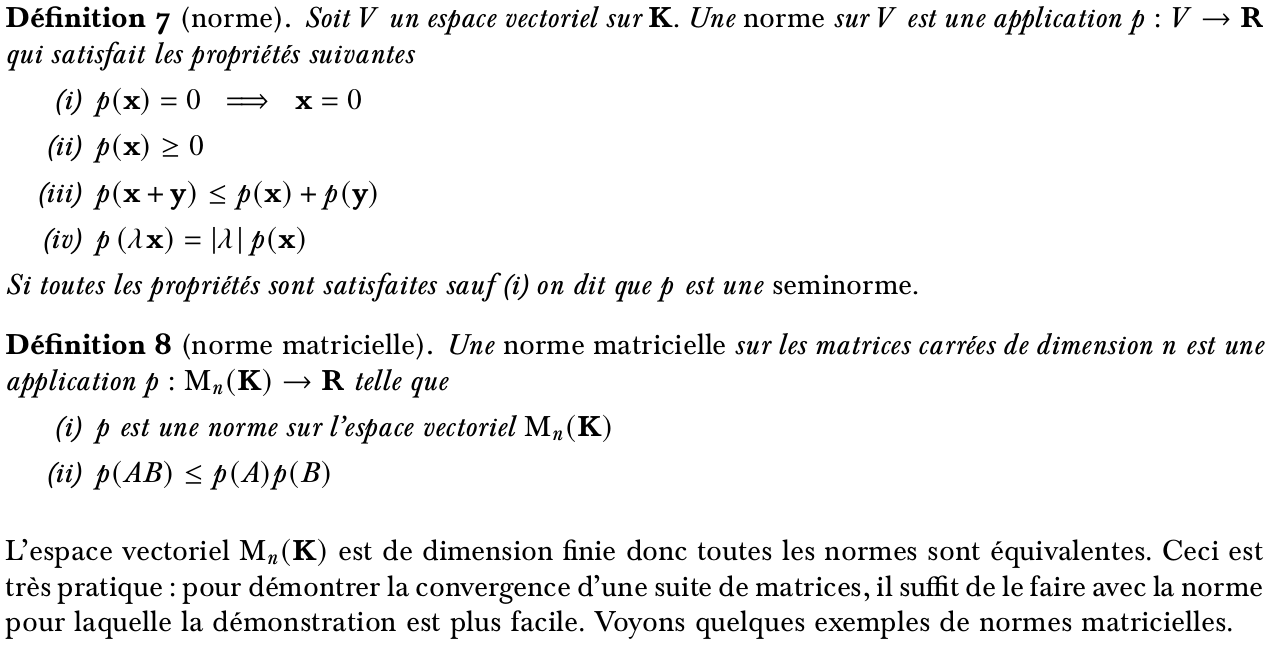
\includegraphics[width=0.98\paperwidth]{f/normesmatricielles.png}
}
\vfill

\end{frame}

% normes matricielles, définition, propriétés, exemples
\begin{frame}
NORMES INDUITES\\
===============

\vfill
\hspace*{-2.3em}\makebox[1\paperwidth][c]{
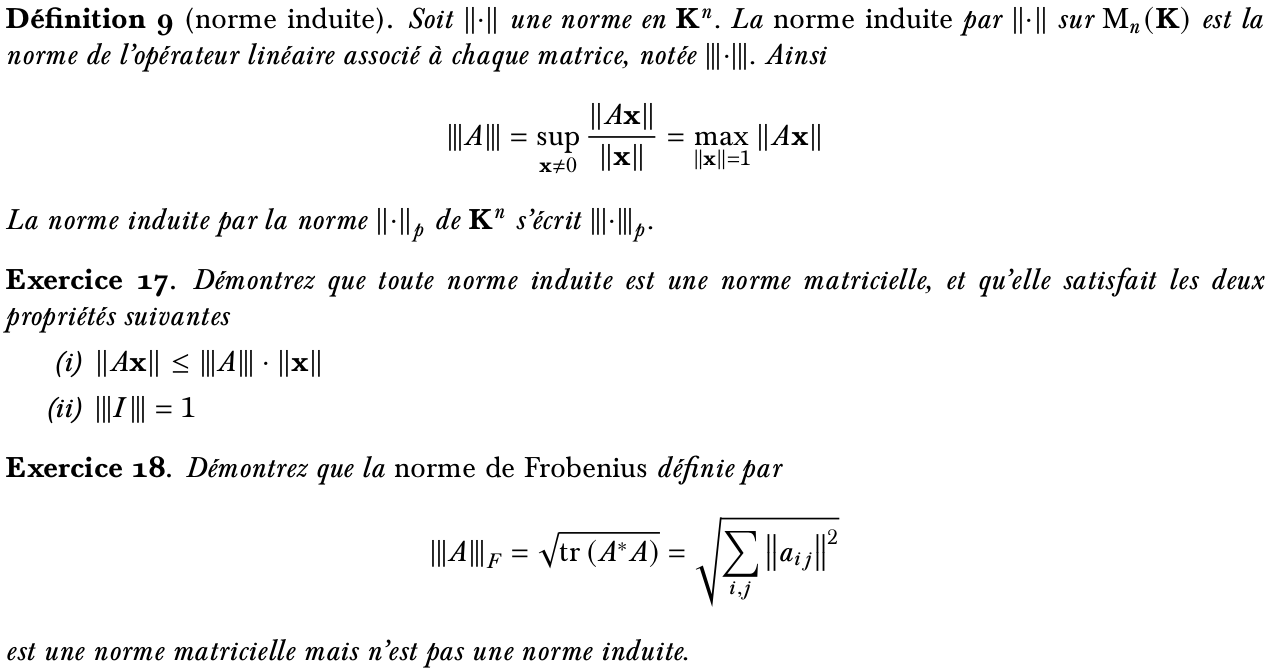
\includegraphics[width=0.98\paperwidth]{f/normesinduites.png}
}
\vfill
\small
\color{red}{\bf Exercice 18:}
démontrez que $\ABS{\cdot}_F$ est une norme matricielle.

\end{frame}

% normes induites classiques
\begin{frame}
NORMES INDUITES CLASSIQUES\\
==========================

{\color{red}{\bf Exercice 19:} démontrez les caractérisations suivantes:}
	\[
		\ABS A_1      = \max_j\sum_i\abs{a_{ij}}
		\qquad
		\ABS A_\infty = \max_i\sum_j\abs{a_{ij}} %= \ABS{A^*}_1
		\qquad
		\ABS A_2      = \sqrt{\rho\parens{A^*A}} %= \ABS{A^*}_2
	\]


\end{frame}

% normes et rayon spectral
\begin{frame}
NORMES ET RAYON SPECTRAL\\
========================

{\color{red}\bf Exercice 20:} Démontrez que\\
	\begin{enumerate}
		\item $\forall A\in\M_n(\K):$~$\rho\parens{A^m}=\rho\parens{A}^m$ et~$\rho\parens{\lambda
			A}=\abs\lambda\rho\parens{A}$
		\item Si~$A$ est diagonale alors~$\ABS A_p=\rho(A)$
			%pour~$1\le p\le\infty$.
		\item Si~$A$ est normale alors~$\ABS A_2=\rho(A)$.
		\item Si~$n>1$ alors~$\rho$ n'est pas une norme matricielle
			%sur~$\M_n(\K)$.
		\item Si~$\ABS\cdot$ est une norme induite sur~$\M_n(\C)$ alors
			\begin{equation}\label{eq:rholessthanABS}
				\rho(A)\le\ABS A
			\end{equation}
		\item L'équation~(\ref{eq:rholessthanABS}) est encore vraie pour
			une norme matricielle quelconque sur~$\M_n(\C)$, ou même
			sur~$\M_n(\R)$.
	\end{enumerate}
	\pause

{\color{red}\bf Exercice 21:} (théorème de Householder)\\
	Pour toute matrice~$A\in\M_n(\C)$ et tout~$\epsilon>0$ il existe une norme
	induite~$\ABS\cdot_{A,\epsilon}$ telle que
	\begin{equation}\label{eq:rhomorethanABS}
		\ABS A_{A,\epsilon}\le\rho(A)+\epsilon
	\end{equation}
\end{frame}

% théorème de Houseolder
\begin{frame}
THÉORÈME DE HOUSEHOLDER\\
=======================

\vfill
\hspace*{-2.3em}\makebox[1\paperwidth][c]{
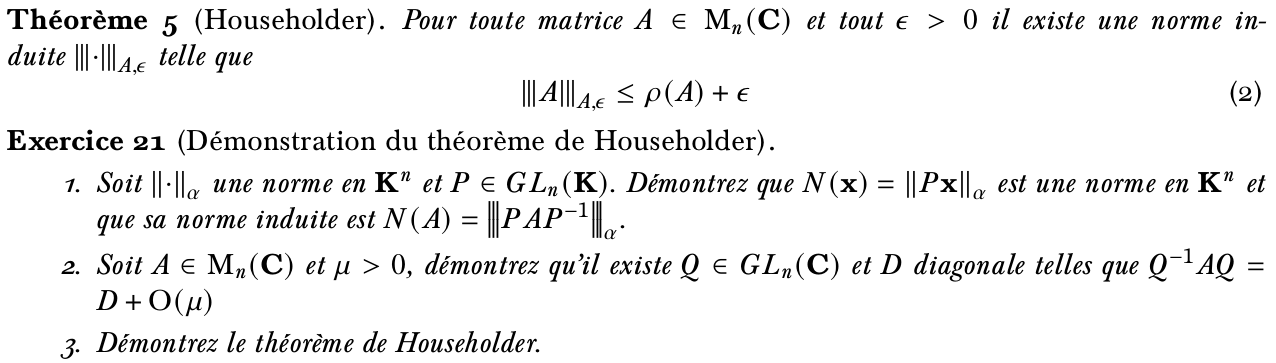
\includegraphics[width=0.98\paperwidth]{f/thhouseholder.png}
}
\vfill
\end{frame}

% convergence de suites de matrices
\begin{frame}
CONVERGENCE DE SUITES DE MATRICES\\
=================================

\vfill
\hspace*{-2.3em}\makebox[1\paperwidth][c]{
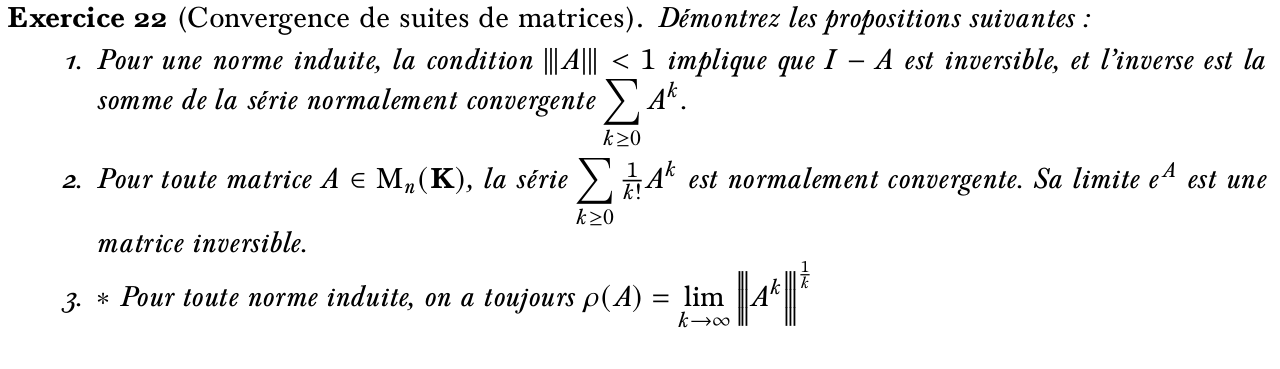
\includegraphics[width=0.97\paperwidth]{f/convsuitmat.png}
}
\vfill
\end{frame}

% conditionement, erreurs d'observation et de modélisation
\begin{frame}
CONDITIONNEMENT DE MATRICES\\
===========================

\vfill
\hspace*{-2.3em}\makebox[1\paperwidth][c]{
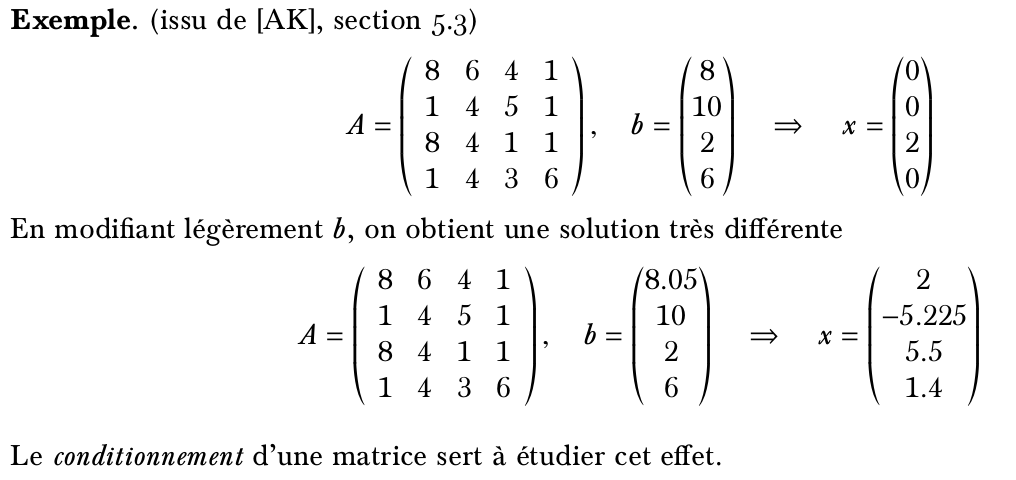
\includegraphics[width=0.97\paperwidth]{f/coditionex.png}
}
\vfill

\end{frame}

\begin{frame}
CONDITIONNEMENT DE MATRICES\\
===========================

{\bf Définition (conditionnement):}
Soit~$A\in\GL_n(\K)$ et~$\ABS\cdot_\alpha$ une norme induite.  Le
\emph{conditionnement} de~$A$ relatif à cette norme est
\[
	\mathrm{cond}_\alpha(A) = \ABS{A}_{\alpha}\ \ABS{A^{-1}}_\alpha
\]

\pause
{\bf Prop. (conditionnement euclidien):} Pour~$A\in\GL_n(\K)$ on a
\[
\mathrm{cond}_2(A) = \sqrt{\frac{\lambda_{\max}(A^*A)}{\lambda_{\min}(A^*A)}}
\]
Si $A$ est normale
\[
\mathrm{cond}_2(A) = \frac{\abs{\lambda_{\max}(A)}}{\abs{\lambda_{\min}(A)}}
\]
Si $O \in U_n(\K)$ alors
\[
\mathrm{cond}_2(O) = 1, \quad \mathrm{cond}_2(AO) = \mathrm{cond}_2(OA) = \mathrm{cond}_2(A)
\]
\end{frame}

\begin{frame}
EFFET DES ERREURS\\
=================

On veut résoudre~$Ax=b$ mais on connait~$b$ (ou~$A$) à des erreurs près.  Quel
est l'effet sur la solution~$x$?
\pause

{\color{red}{\bf Exercice 23:} (erreurs d'observation)}
Si~$A(x+\delta x)=b+\delta b$ alors
	\[
		\frac{\Abs{\delta x}}{\Abs{x}}
		\le
		\mathrm{cond}(A)
		\frac{\Abs{\delta b}}{\Abs{b}}
	\]

\pause
{\color{red}{\bf Exercice 24:} (erreurs de modélisation)}
Si~$(A+\delta A)(x+\delta x)=b$ alors
	\[
		\frac{\Abs{\delta x}}{\Abs{x+\delta x}}
		\le
		\mathrm{cond}(A)
		\frac{\ABS{\delta A}}{\ABS{A}}
	\]

	Ces deux inégalités sont {\bf\color{red}optimales}.
\end{frame}

\begin{frame}
ERREURS DE CONDITIONNEMENT\\
=========================

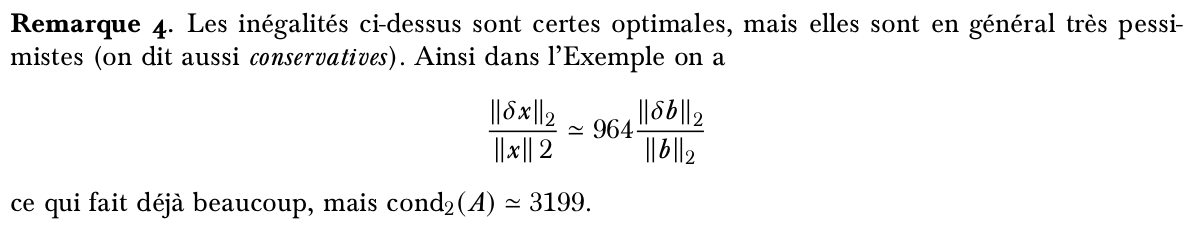
\includegraphics[width=\linewidth]{f/erreursoptimales.png}
\end{frame}

\begin{frame}
PRÉCONDITIONNEMENT\\
==================


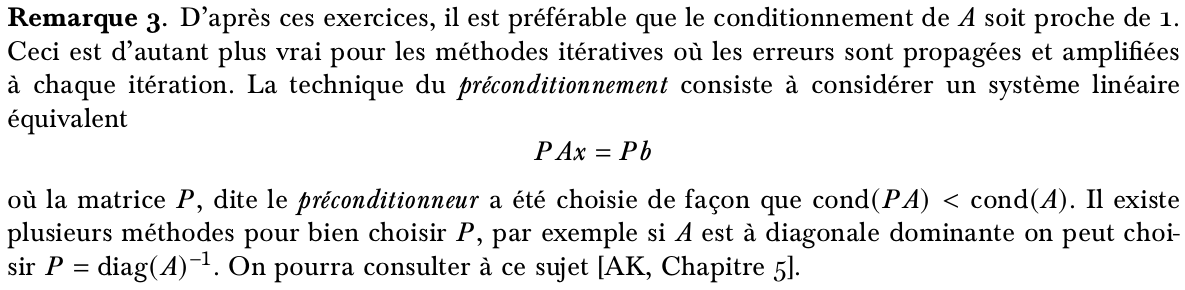
\includegraphics[width=\linewidth]{f/precond.png}
\end{frame}



% complexité (def)
\begin{frame}
COMPLEXITÉ (DÉFINITION)\\
=======================

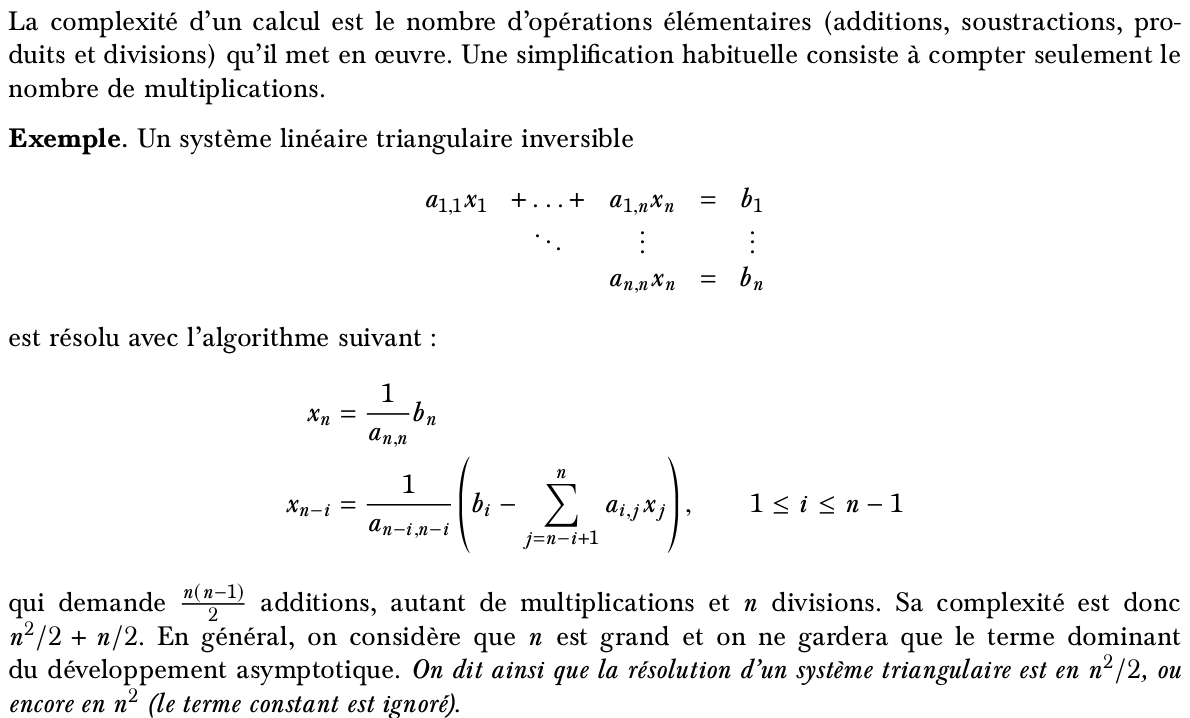
\includegraphics[width=\linewidth]{f/complexdef.png}
\end{frame}

% complexité (exercice)
\begin{frame}
COMPLEXITÉ (EXEMPLES)\\
=====================


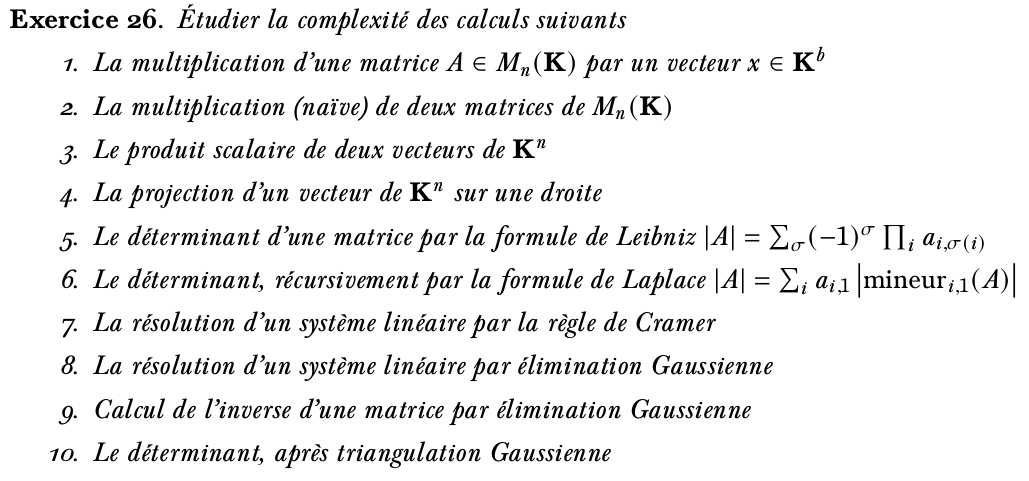
\includegraphics[width=\linewidth]{f/complexex.png}
\end{frame}


% complexité (multiplications)
\begin{frame}
MULTIPLICATION DE WINOGRAD\\
==========================

{\footnotesize\color{blue}
\[
	\begin{pmatrix}
		a & b \\ c & d
	\end{pmatrix}
	\begin{pmatrix}
		A & C \\ B & D
	\end{pmatrix}
	=
	\begin{pmatrix}
		aA+bB & w+v+(a+b-c-d)D \\
		w+u+d(B+C-A-D) & w+u+v
	\end{pmatrix}
\]
}

$u=(c-a)(C-D)$\\
$v=(c+d)(C-A)$\\
$w=aA+(c+d-a)(A+D-C)$.\\
Ce calcul entraîne~$7$ multiplications et~$15$ additions.

\pause
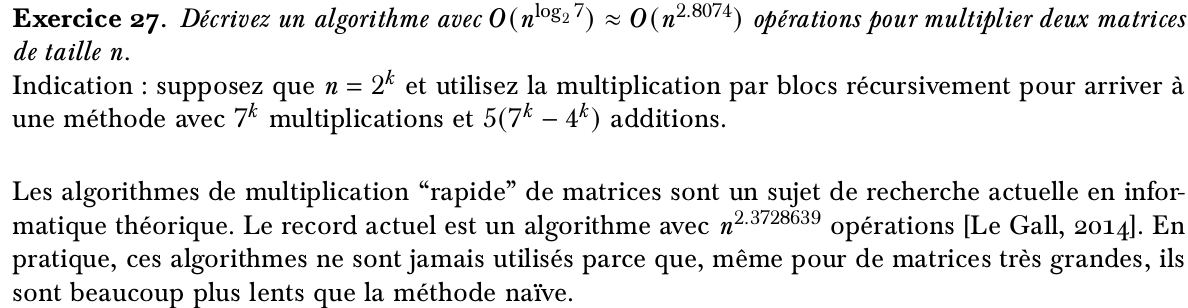
\includegraphics[width=\linewidth]{f/fastmult.png}
\end{frame}


% complexité: commentaires
\begin{frame}
COMPLEXITÉ: COMMENTAIRES {\bf EN 2020}\\
================================

1. En pratique, 1 produit $\approx$ 1 addition

2. La performance dépend surtout d'un accès ordonnée en mémoire qui évite des
``cache faults.''

3. Il est essentiel que l'algorithme soit parallélisable en GPU

4. On ne s'intéresse jamais à la solution exacte théorique, mais au taux
d'approximation des méthodes itératives.

5. Les grandes matrices sont souvent creuses, ce qui requiert un analyse de la
complexité différent (e.g., le produit matrice-vecteur  se fait en temps
linéaire).
\end{frame}


% méthodes directes: gauss
\begin{frame}
MÉTHODE DE GAUSS\\
================

{\bf Idée:}\\
transformer~$Ax=b$ en un système triangulaire équivalent

\pause
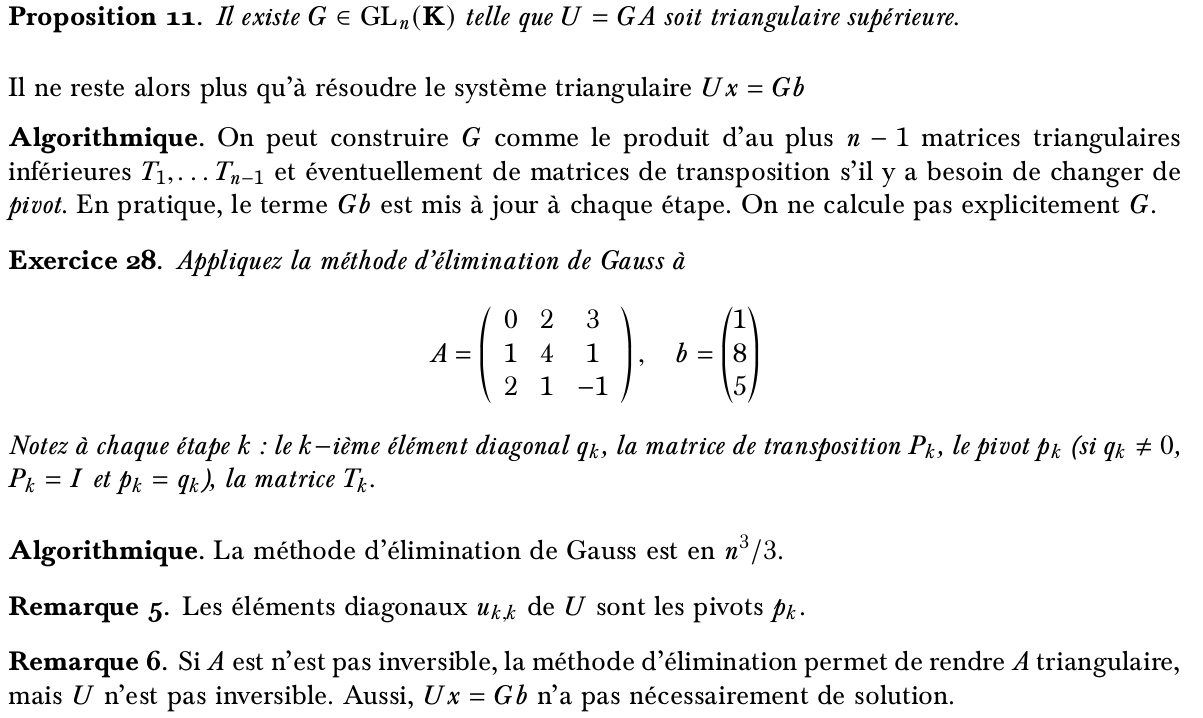
\includegraphics[width=\linewidth]{f/gauss.png}
\end{frame}

% méthodes directes: LU
\begin{frame}
MÉTHODE LU\\
==========

LU = formalisation matricielle de la méthode de Gauss

\pause
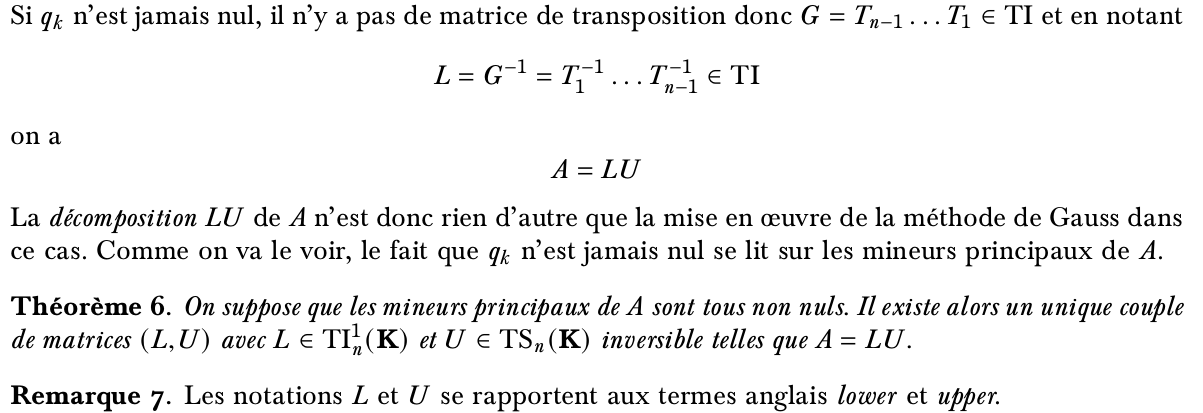
\includegraphics[width=\linewidth]{f/lu.png}

\color{red}\bf Exercice 30: démontrer le théorème ``LU''
\end{frame}

%% méthodes directes: LU exercice
%\begin{frame}
%méthode de gauss\\
%================================
%
%\end{frame}

% méthodes directes: Cholesky
\begin{frame}
MÉTHODE DE CHOLESKY\\
===================

{\bf Théorème 7.}  Soit~$A\in\HH_n^{++}(\C)$, alors il existe une unique~$B\in\TI_n^{++}(\C)$ telle que
\[ A = B B^* \]

{\color{red}{\bf Exercice 32. } Prouver le théorème 7.}

%\begin{enumerate}
%\item Sous réserve d'existence, montrez l'unicité.
%\item Justifiez que $A$ admet une décomposition $LU$ et que les $u_{k,k}$ sont strictement positifs.
%\item On note 
%\[
%D = \left(\begin{array}{ccc}
%\sqrt{u_{1,1}} & & \\
%& \ddots & \\
%& & \sqrt{u_{n,n}}
%\end{array}\right)
%\]
%Montrez que $B = LD$ convient.
%\end{enumerate}

{\color{red}{\bf Exercice 32'. }
Établir la factorisation de Cholesky de la matrice
\[
A = \left(\begin{array}{ccc}
1 & 2 & 1 \\
2 & 13 & 2 \\
 1 & 2 & 2
\end{array}\right)
\]
}
\end{frame}

\begin{frame}
MÉTHODE DE CHOLESKY: IMPLEMENTATION EN C\\
========================================


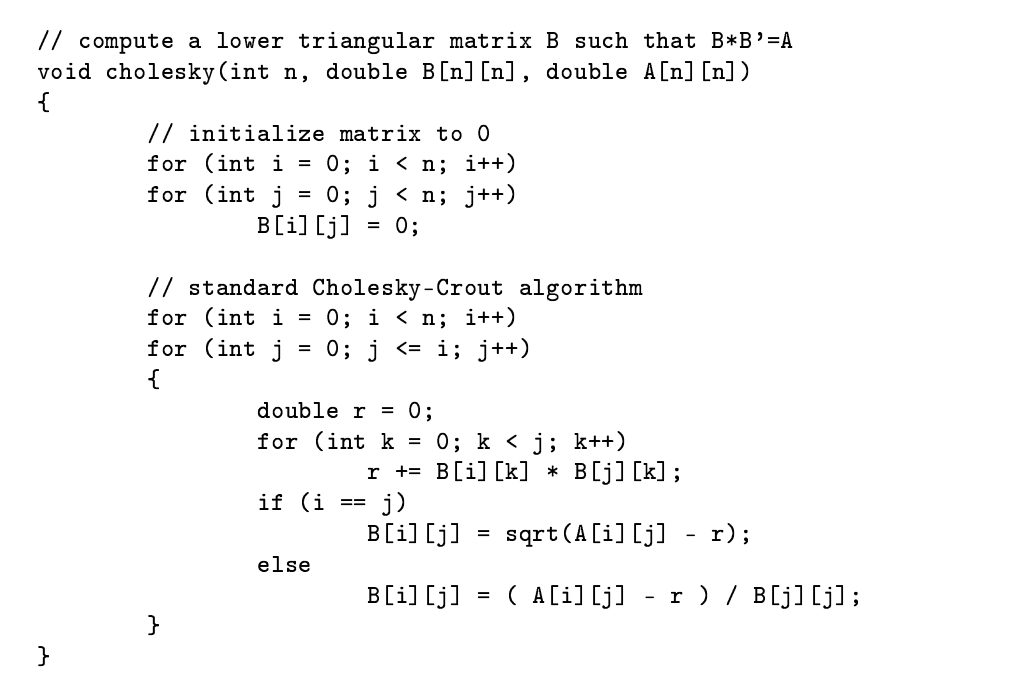
\includegraphics[width=\linewidth]{f/choleskyc.png}
\end{frame}

% méthodes directes: QR
\begin{frame}
MÉTHODE QR\\
==========

{\bf Théorème 8.}
Soit $A \in\GL_n(\K)$. Il existe un unique couple de matrices $(Q,R)$ avec $Q
\in \UU(n)$ et $R \in \TS^{++}_n(\K)$ telles que
\[
A = QR
\]
Ceci définit un homéomorphisme de $\GL_n(\K)$ sur $\UU(n)\times\TS^{++}(\K)$.

{\color{red}{\bf Exercice 34. } Prouver le théorème 8.}
\end{frame}

% méthodes directes: exemples
\begin{frame}
EXEMPLES DE FACTORISATIONS\\
==========================


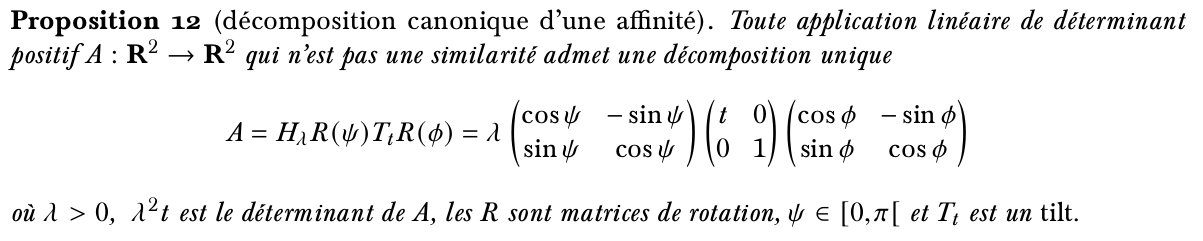
\includegraphics[width=\linewidth]{f/prop12.png}

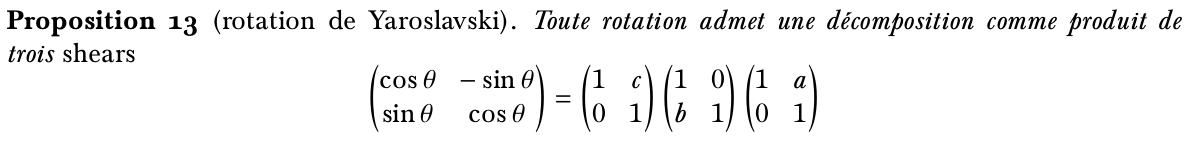
\includegraphics[width=\linewidth]{f/prop13.png}

\pause
{\color{red}{\bf Exercice 35.} Démontrez les propositions 12 et 13.  Pour 13,
	exprimez~$a,b,c$ en fonction de l'angle~$\theta$.
}
\end{frame}


\begin{frame}
REPARTITION DES EXERCICES\\
=========================

%{\bf Tous:} Exercices 1, 2 (intersection de groupes) et 5.\\
%{\bf Groupe 1:} Exercice 3 (théorème spectral)\\
%{\bf Groupe 2:} Exercices 4 et 6 (éléments propres)\\
%{\bf Groupe 3:} Exercice 7 (théorème du min-max)\\
%{\bf Groupe 4:} Exercice 8 et 9 (disques de Gershgorin)\\
%{\bf Groupe 5:} Exercice 12 et 13 (décomposition polaire)\\
%{\bf Groupe 6:} Exercice 14, 15 et 17 (pseudo-inverse)\\
{\bf Groupe 1:} Exercices 18, 19 (normes matricielles)\\
{\bf Groupe 2:} Exercices 20(5), 21 (normes et spectre)\\
{\bf Groupe 3:} Exercice 23, 24 (erreurs et conditionnement)\\
{\bf Groupe 4:} Exercice 32, 32' (Cholesky)\\
{\bf Groupe 5:} Exercice 34 (QR)\\
{\bf Groupe 6:} Exercice 35 (affinités et rotations)\\


\vfill
Temps:\\
{\bf 90min} travail en groupe (6 groupes de 2,3 personnes)\\
{\bf 60min} mise en commun
(6 présentations de 10min par les ``scribes'' de chaque groupe)

\end{frame}

\end{document}


% vim:sw=2 ts=2 spell spelllang=fr:
